%%%%%%%%%%%%%%%%%%%%%%%%%%%%%%%%%%%%%%%%%
% YOMAMA litepaper
%%%%%%%%%%%%%%%%%%%%%%%%%%%%%%%%%%%%%%%%%

\documentclass[11pt]{scrartcl} % Font size

\usepackage{amsmath, amsfonts, amsthm} % Math packages


\usepackage{listings} % Code listings, with syntax highlighting


\usepackage[english]{babel} % English language hyphenation

\usepackage{graphicx} % Required for inserting images
\graphicspath{{Figures/}{./}} % Specifies where to look for included images (trailing slash required)

\usepackage{booktabs} % Required for better horizontal rules in tables

\numberwithin{equation}{section} % Number equations within sections (i.e. 1.1, 1.2, 2.1, 2.2 instead of 1, 2, 3, 4)
% \numberwithin{figure}{section} % Number figures within sections (i.e. 1.1, 1.2, 2.1, 2.2 instead of 1, 2, 3, 4)
\numberwithin{table}{section} % Number tables within sections (i.e. 1.1, 1.2, 2.1, 2.2 instead of 1, 2, 3, 4)

\setlength\parindent{0pt} % Removes all indentation from paragraphs

\usepackage{enumitem} % Required for list customisation
\setlist{noitemsep} % No spacing between list items

\usepackage{geometry} % Required for adjusting page dimensions and margins

\geometry{
	paper=a4paper, % Paper size, change to letterpaper for US letter size
	top=2.5cm, % Top margin
	bottom=3cm, % Bottom margin
	left=3cm, % Left margin
	right=3cm, % Right margin
	headheight=0.75cm, % Header height
	footskip=1.5cm, % Space from the bottom margin to the baseline of the footer
	headsep=0.75cm, % Space from the top margin to the baseline of the header
	%showframe, % Uncomment to show how the type block is set on the page
}

\usepackage[utf8]{inputenc} % Required for inputting international characters
\usepackage[T1]{fontenc} % Use 8-bit encoding

% \usepackage{fourier} % Use the Adobe Utopia font for the document

\usepackage{sectsty} % Allows customising section commands

\sectionfont{\vspace{6pt}\centering\normalfont\scshape} % \section{} styling
\subsectionfont{\normalfont\bfseries} % \subsection{} styling
\subsubsectionfont{\normalfont\itshape} % \subsubsection{} styling
\paragraphfont{\normalfont\scshape} % \paragraph{} styling


\usepackage{scrlayer-scrpage} % Required for customising headers and footers

\ohead*{} % Right header
\ihead*{} % Left header
\chead*{} % Centre header

\ofoot*{} % Right footer
\ifoot*{} % Left footer
\cfoot*{\pagemark} % Centre footer
 % Include the file specifying the document structure and custom commands

\title{	
	\normalfont\normalsize
	\textsc{Yomama so fat, her litepaper spans 69 volumes}\\ 
}

\author{\LARGE YOMAMA} % Your name

\date{\normalsize\today} % Today's date (\today) or a custom date

\begin{document}

\maketitle % Print the title

\begin{figure}[h] % [h] forces the figure to be output where it is defined in the code (it suppresses floating)
	\centering
	
\includegraphics[width=0.5\columnwidth]{yomama.png} % Example image
	\caption{This is Yomama.}
\end{figure}

%------------------------------------------------

\section{Introduction}

Yomama got so fat from eating all the food tokens, that she grew into a hybrid model between three of the hottest things in defi right now: staking, token burn and yield farming. Everything is set up to hugely inflate price from the start. You know Yomama likes to bang.

\section{YOMA tokenomics}

Max supply is \textbf{20,000 YOMA}
\begin{itemize}
	\item 9,800 (49\%) is locked for Yield Farming rewards
	\item 7,000 (35\%) YOMA is going to public presale
	\item 2,500 (12,5\%) YOMA for intitial liquidity on Uniswap at 2.8x the presale price
	\item 500 (2,5\%) YOMA will be allocated to team
	\item 200 (1\%) YOMA will be used for promotions
\end{itemize}

\section{Token Model}

\subsection{Token burn}

Yomama loves it when you buy and use her, so you can buy and transact without burn. BUT, she gonna get real mad when you sell! So each time tokens are sold on Uniswap, part of sold tokens get "burned" directly into the staking pool where they will be distributed over the good boys that stake YOMA.

The burn curve will have a half-life of 1 day, and will plateau after 4 days. The burn percentage is determined as follows:

\begin{equation} 
	\label{eq:burn}
		b(t)=
	\begin{cases}
		\frac{50}{2^{t/86400}}, & \text{if } t\leq 345600\\
		3.125	& \text{if } t > 345600
	\end{cases}					
\end{equation}

Where t is the time in seconds since the blocktime of the Uniswap listing.

\begin{figure}[h] % [h] forces the figure to be output where it is defined in the code (it suppresses floating)
	\centering
	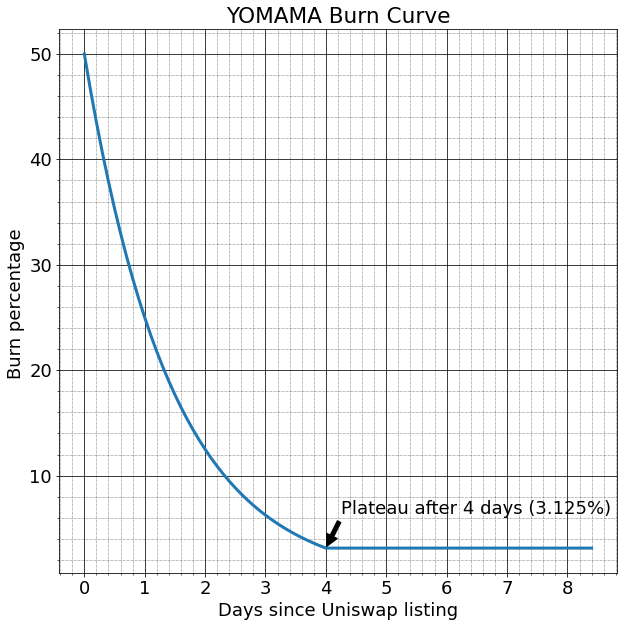
\includegraphics[width=0.5\columnwidth]{burn_curve.png} % Example image
	\caption{Look at Yomama's burn curve.}
\end{figure}

The burn mechanism on sell will hugely inflate YOMAMA ('s price) on listing, and will reward YOMA stakers.

\subsection{Staking}

Good boys know how annoying it can be, you buy a token, and then have to spend ETH again to provide liquidity. We have a solution - You can simply stake your YOMA tokens on our dashboard and earn staking rewards. Staking rewards are generated from the token burn and are distributed proportionally to YOMA stakers. Our dashboard will provide insights in your rewards, and will have an option to instantly restake rewards.

\subsection{Yield Farming}

Good boys know how annoying it can be, you buy a token, and then have to spend ETH again to provide liquidity. We have a solution - You can simply stake your YOMA tokens on our dashboard and earn staking rewards. Staking rewards are generated from the token burn and are distributed proportionally to YOMA stakers. Our dashboard will provide insights in your rewards, and will have an option to instantly restake rewards.

Yield farming is a juicy way to earn some YOMA, we are starting off with a huge APY, just like YOMAMA. 
The yield farming average daily APY is determined by the following equations:

\begin{equation} 
	\label{eq:yieldemission}
		emission(d)= 
		\frac{\partial}{{\partial d}} (9800-\frac{9800}{2^{\frac{d}{7}}})
\end{equation}

and, using a listing price of 2.8x and assuming half of the people use their tokens to yield farm: (3500 tokens) we get

\begin{equation} 
	\label{eq:yieldapy}
		APY(d)= 
		\frac{100*2.8*365*d}{3500}
\end{equation}

The yield farming APY curve looks like this

\begin{figure}[h] % [h] forces the figure to be output where it is defined in the code (it suppresses floating)
	\centering
	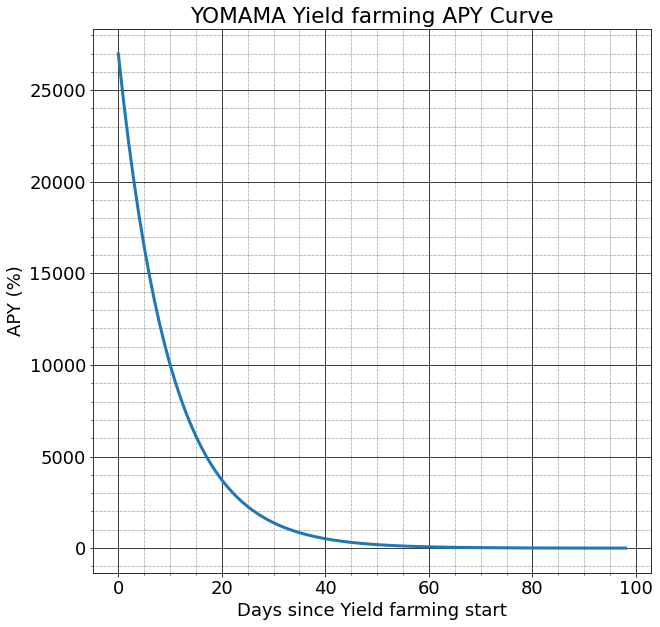
\includegraphics[width=0.5\columnwidth]{yield_curve.png} % Example image
	\caption{This is Yomama's yield farming APY curve.}
\end{figure}

\clearpage

\subsubsection{Yield APY}

For the first 30 days the daily average APY will be:

\begin{table*}[h] % [h] forces the table to be output where it is defined in the code (it suppresses floating)
	\centering % Centre the table
	\begin{tabular}{p{2cm} p{2cm}}
		\toprule
		\textit{Day} & \textbf{APY} \\
		\bottomrule
		Day 0 & 26978\%\\
		Day 1 & 24435\%\\
		Day 2 & 22131\%\\
		Day 3 & 20045\%\\
		Day 4 & 18155\%\\
		Day 5 & 16443\%\\
		Day 6 & 14893\%\\
		Day 7 & 13489\%\\
		Day 8 & 12217\%\\
		Day 9 & 11066\%\\
		Day 10 & 10022\%\\
		Day 11 & 9077\%\\
		Day 12 & 8222\%\\
		Day 13 & 7447\%\\
		Day 14 & 6745\%\\
		Day 15 & 6109\%\\
		Day 16 & 5533\%\\
		Day 17 & 5011\%\\
		Day 18 & 4539\%\\
		Day 19 & 4111\%\\
		Day 20 & 3723\%\\
		Day 21 & 3372\%\\
		Day 22 & 3054\%\\
		Day 23 & 2766\%\\
		Day 24 & 2506\%\\
		Day 25 & 2269\%\\
		Day 26 & 2055\%\\
		Day 27 & 1862\%\\
		Day 28 & 1686\%\\
		Day 29 & 1527\%\\
	\end{tabular}
	\caption{Average daily APY\%}
\end{table*}

\end{document}
